\textcolor{violet}{\section{Design For Manufacture And Assembly}}

\subsection{Design For Assembly}

Our current idea for creating smart lock is having a pinpad on the front along with either a camera or fingerprint scanner on the top of the lock. Inside the lock, we have an ESP32-C3 microcontroller that connects to the wifi and the server. Our current design is shown below as a non functioning prototype, meant for aesthetics.

% Information about side-to-side figures:
% https://tex.stackexchange.com/questions/37581/latex-figures-side-by-side
\begin{figure}[htbp]
    \centering
    \begin{subfigure}[b]{0.48\textwidth}
        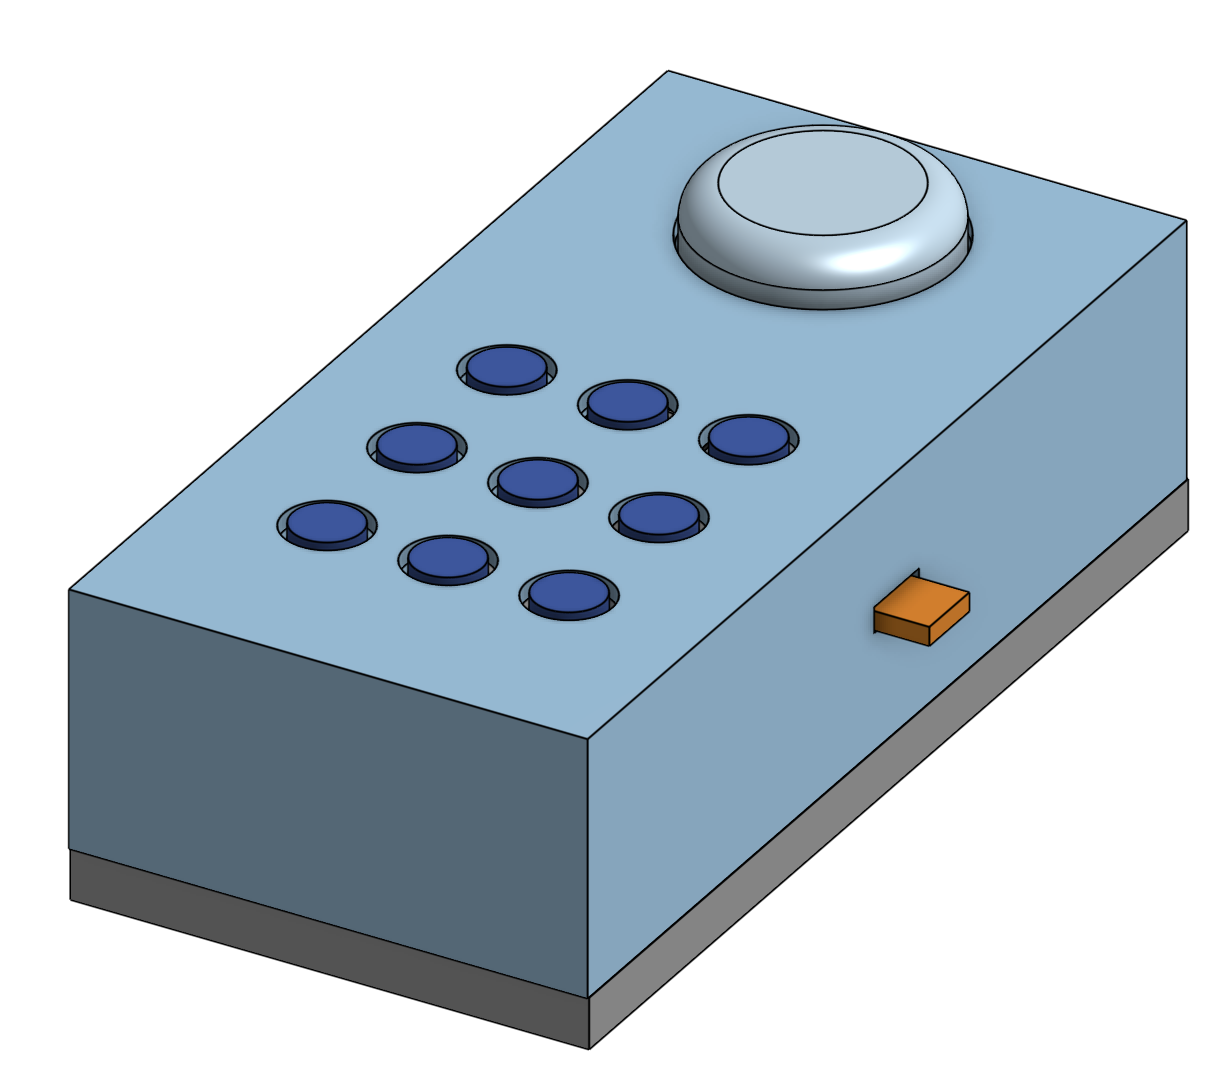
\includegraphics[width=\textwidth]{./img/isoView.png}
        \caption{Isometric View}
        \label{fig:isoView}
    \end{subfigure}
    \hfill
    \begin{subfigure}[b]{0.48\textwidth}
        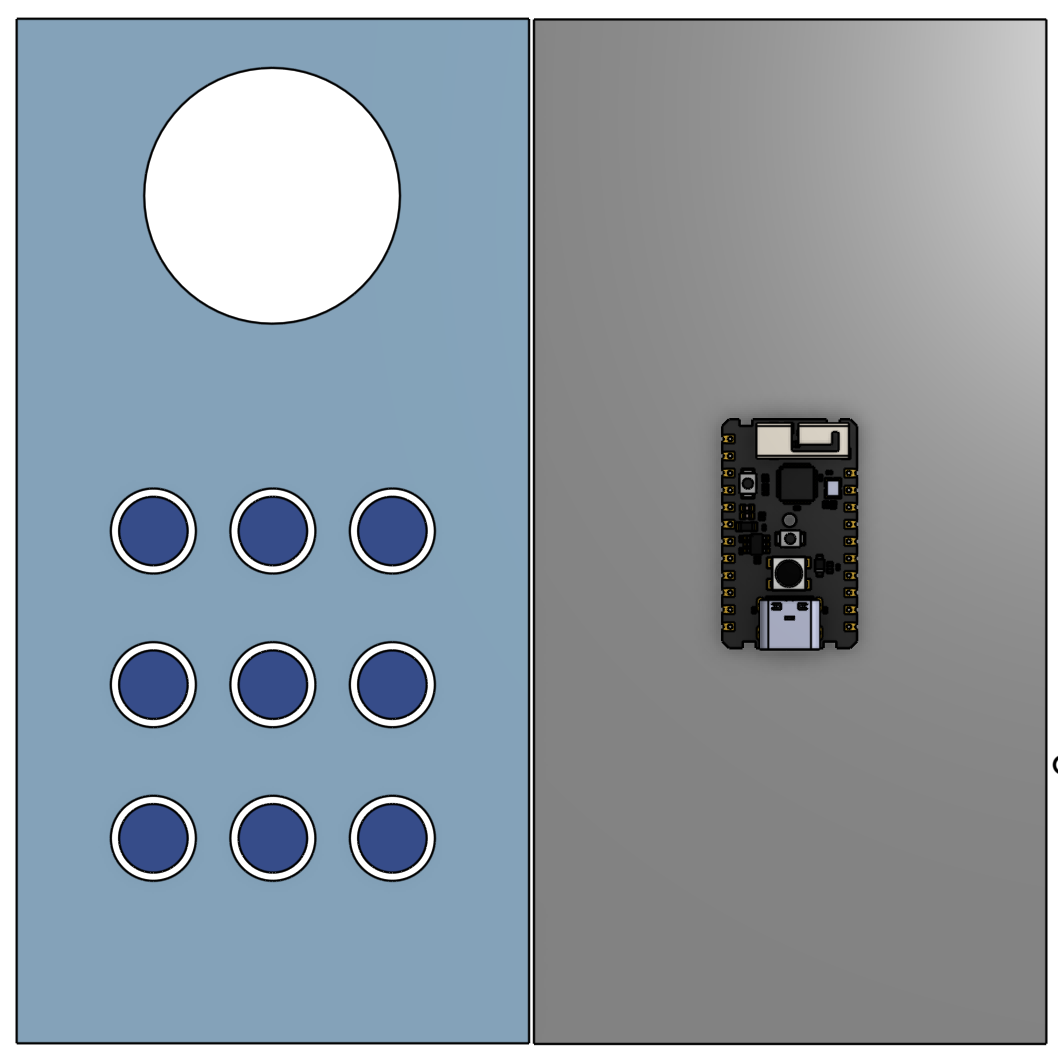
\includegraphics[width=\textwidth]{./img/topView.png}
        \caption{Top View}
        \label{fig:topView}
    \end{subfigure}
    \caption{First lock design}
\end{figure}

The most basic functionality that our lock needs to do is being able to send information to the lock from a device to the lock, telling it to either lock or unlock the door. As we slowly develop our smart lock, we will be able to add in more functionalities such as generating pin codes for the pincode lock. By the end of Winter 2025 quarter, we can prove that our phone and microcontroller is able to connect to the server to tell the lock to either unlock or lock the door.

\newpage
\textcolor{violet}{\subsection{Design For Manufacture} \label{DesignForManufacture}}

The manufacturing layout of the prototype below displays all the necessary components to provide a foundation for our main design. The components shown in the diagram are the most cost-efficient and power-efficient parts to achieve a functioning auto-locking door.

\begin{figure}[!ht]
    \centering
    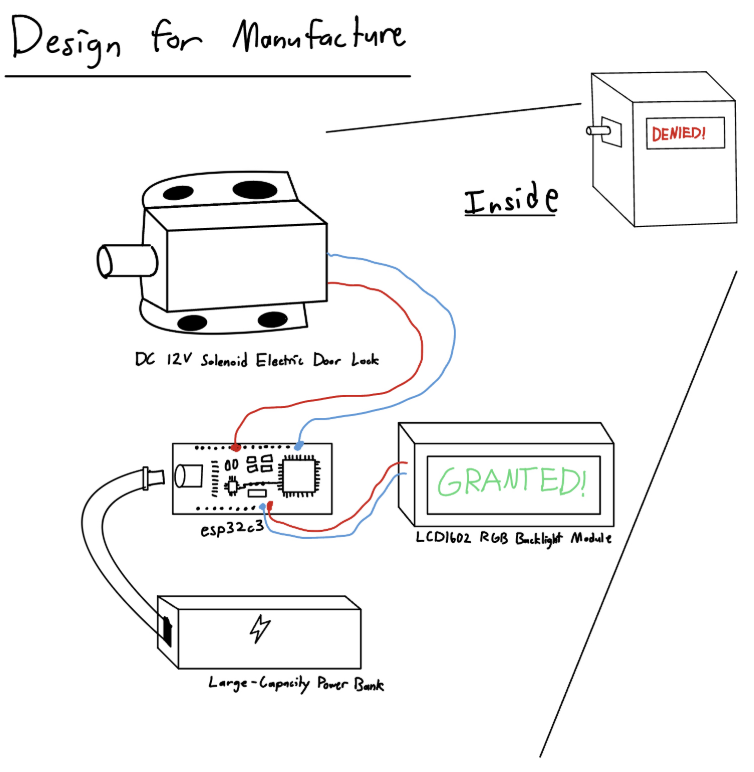
\includegraphics[width=0.85\linewidth]{./img/DFM.png}
    \caption{Necessary Components}
    \label{fig:enter-label}
\end{figure}

The prototype components shown in the diagram above display a DC 12V Solenoid Electric Door Lock, an esp32c3, LCD1602 RGB Backlight Module V1.0, a Large-Capacity Power Bank, a USB-C cable, standard Male-to-Female wires, and a 3D printed container for all the components to fit together. A budget list for the items will be provided on the following page.

\newpage
